\section{Hardware lag}
I det kommende afsnit vil den valgt hardware konfiguration gennemgås. 
Den dybere tekniske beskrivelse i forhold til produkt specifikke registre eller anden speciel arkitektur, vil ikke i detaljer beskrives, med mindre det er en vigtig del af argumentationen for valget.
Det komplette hardware modul findes i \emph{hardware.c}.

\subsection{Valg af hardware profil}
\begin{wrapfigure}{r}{0.4\textwidth}
	\centering
	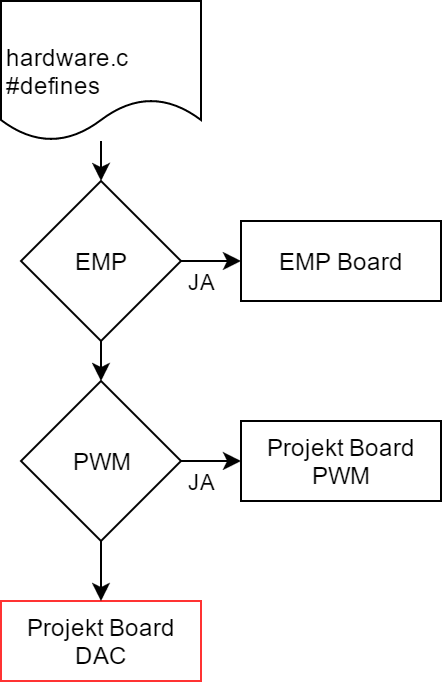
\includegraphics[width=.3\textwidth]{billeder/hardware_profiles.png}
	\caption{Oversigt over mulige konfigurationer af \textit{hardware.c}.}
	\label{fig:hardware_profiler}
\end{wrapfigure}
For at kunne håndtere de forskellige opsætninger af hardware i udviklingsforløbet af equalizerens software, er der lavet forskellige hardware opsætninger, således at man på en nem måde kan skifte imellem dem.
\\
I \textit{global.h} filen, findes to compiler \textbf{\#define} direktiver til makro definitionerne \textbf{EMP} og \textbf{DAC}.
Sammenhænget mellem profilerne ses i figur \ref{fig:hardware_profiler}. 
Således kan man teste softwaren på EMP printet, med den monterede mikrofon indgang og hovedtelefon udgang, ved at vælge \textbf{EMP} profilen.
Fravælges \textbf{EMP} profilen, skifter softwaren over til at bruge projekt printet.
Her kan der vælges imellem DAC eller PWM som udgangssignal.  
Den tilhørende pin-konfiguration for de valgte hardware profiler kan ses i bilag \ref{bilag:pinmap}.

\subsection{ADC}

\jj{Adc afsnit skal komme her lige før SPI/DAC ( således overgang fra lyd input til lyd output)}


\subsection{PWM}
\husk{jj}{Gennegang af PWM på EMP. }
\husk{jj}{PWM til projekt.}
\husk{jj}{Noter til PWM : PWM opløsning, fase korrect signal. Se om der kan findes information mht. en PWM frekvens på ca. 10 gange signal frekvensen.}
\husk{jj}{Segway til DAC.}
\husk{jj}{Kom kort ind på de uhensigtmæssige signal fejl ved PWM i forhold til måling og bestemmelse af EQ's effektivitet.}

\subsection{DAC}
Til at generer udgangssignalet fra MCU'en vælges en ekstern DAC kreds, da MCU'en ikke råder over denne funktionalitet.
Valget blev en \texttt{MCP4922E/P}\footnote{Microchip MCP4922E/P 12-Bit Dual Voltage Output Digital-to-Analog Converter with SPI Interface \cite{mcp4922} } 12bit DAC , så at opløsningen på udgangen er den sammen som på indgangen.
Således er spændingsdifferencen for den mindst betydende bit $ V_{LSb} = V_{ref} / 4096 \approx \num{0,8}\si{\milli\volt} $, ved en ekstern reference spænding på $V_{ref} = 3,3\si{\volt}$.
Derudover har den valgte DAC en maksimal indsvingningstid på $t_{settling} = \num{4.5}\si{\micro\second}$, hvilket passer fint til samplingsperioden på $23\si{\micro\second}$. 
\jj{Hvis der bliver plads kan AC fejl i DACøen beskrives her }

\subsection{SPI}
Den valgte DAC forbindes direkte til MCU'en igennem en SPI bus, de valgte pins er beskrevet i bilag \ref{bilag:pinmap}.
Ifølge databladet er datakommunikation på optil $20\si{\mega\hertz}$ mulig, men SPI port konfigurationen på MCU'en sættes til $10\si{\mega\hertz}$.
For at sætte den ønskede udgangsspænding på DAC'en, er en 16 bit kommando nødvendig. 
I figur \ref{fig:dac12bit_writecmd} ses den nødvendige bitsekvens.
En $10\si{\mega\hertz}$ giver således en kommando overføringstid på $t_{cmd}$ for begge lydkanaler på minimum 
\begin{align}
	t_{cmd} = \frac{N_{kanal} \cdot 16bit}{F_{CLK}} = \frac{2 \cdot 16}{10\si{\mega\hertz}} = 3\si{\micro\second}
\end{align}

\begin{figure}[h!]
	\centering
	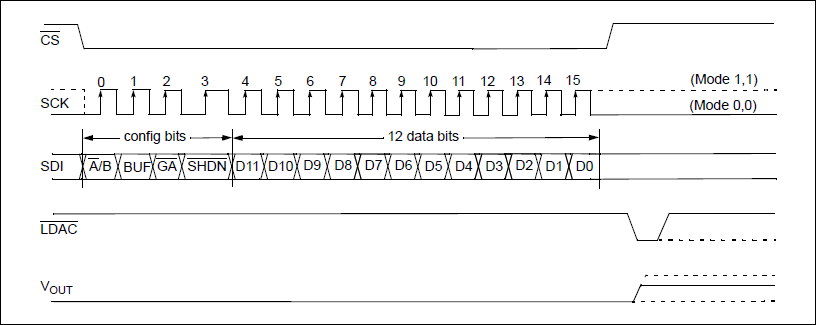
\includegraphics[width=.8\textwidth]{billeder/dac12bit_writecmd.png}
	\caption{Skrive kommando til 12bit MCP4922 DAC.\cite[s. 25]{mcp4922}}
	\label{fig:dac12bit_writecmd}
\end{figure}

I overensstemmelse med databladene for DAC'en og MCU'en, bruges SPI Freescale Fame formatet \footnote{Se afsnit 15.3.4 \cite[s. 954]{tm4c123gh6pm}} i \textbf{Mode 0,0}.

\jj{beskriv AB, BUF, GA og SHDN}

Konfigurationen af SPI laves i \texttt{spi\_init()} i modulet \textit{hardware.c}

\jj{Beskrive LDAC funktionalitet}   

\FloatBlock



\subsection{UART}
\jj{Meget kort beskrivelse af opsætning af uart til den ønskede baudrate.}

\subsection{LCD}
\jj{LCD konfiguratoin er arvet fra EMP board, men det er i drift ikke noget krav at der bruges et LCD, således bør det kunne fjernes ved et release build og kun brugbart ved udvikling
}
\subsection{TIVA}
\jj{Kort beskrivelse af Tiva Board konfiguration, med henvisninger til release note for produktet.}

\subsection{FPU}
\jj{Beskrivelse af produkt specifik aktivering af FPU med henvisning til TI dokumentation. }

\subsection{Interrupt}


\subsection{sysTick og Timers}


\subsection{ADC fra Simon}
En analog til digital konverter kan anvendes til at konvertere et sammenhængende analogt spændingssignal til et diskret digitalt nummer. TMC4C123GH6PM microcontrolleren har to identiske 12 bit A/D konvertere indbygget - ADC0 og ADC1. Det konverterede signal, kan derefter behandles vha. digitale signalbehandlingsmetoder. 
Da der ønskes at opbygge en stereostyret equalizer, bruges begge A/D konvertere. Konfigurationen er derfor ens på hhv. ADC0 og ADC1. Begge A/D konvertere kører uafhængigt af hinanden. Afhængig af hvilken Sample frequencer der er valgt, gemmes
resultatet af A/D konverteringen i et FIFO register (first in - first out). Da der kun er brug for én sample ad gangen, vælges ud fra databladet at konfigurere A/D konverterne med Sample sequencer 3, og derved gemmes resultatet af konverteringen også i ADCSSFIFO3 registeret for hhv. ADC0 og ADC1.
Da det ikke er alle porte, der kan anvendes på microcontrolleren til A/D konvertering, er pin PB5 valgt til at styre venstre kanal, og pin PE4 er valgt til at styre højre kanal. Herudover kan den også køre i mono, frem for stereo - denne er konfigureret på pin PE5. Der ønskes en samplingsfrekvens på $44,1\si\kilo\hertz$ for at undgå aliasing. Denne samplingsfrekvens er bestemt ud fra Nyquist frekvensen. For at få denne samplingsfrekvens korrekt, skal microcontrollerens CPU frekvens sættes til $80\si\mega\hertz$. Der bruges et PWM signal, som er interruptstyret. Dette signal skal køre et bestemt antal cycles.

\begin {equation}
\text{Cycles} = \frac{\text{CPU frekvens}}{\text{Sample frekvens}} => \frac{80\cdot 10^6\si\hertz}{44100\si\hertz} = 1814 \text{cycles}
\end {equation}

Hver gang PWM'en har kørt i det beregnede antal cycles, bliver et interrupt initialiseret, og samplingen starter samt gemmer værdien. Ved næste interrupt, starter processen for A/D konverteringen igen.
Da A/D konverterne er opløst i 12 bit, og den maksimale spænding der bliver registreret er $3,3\si\volt$ - vil maksimalværdien for konverteringen være $4096$. 